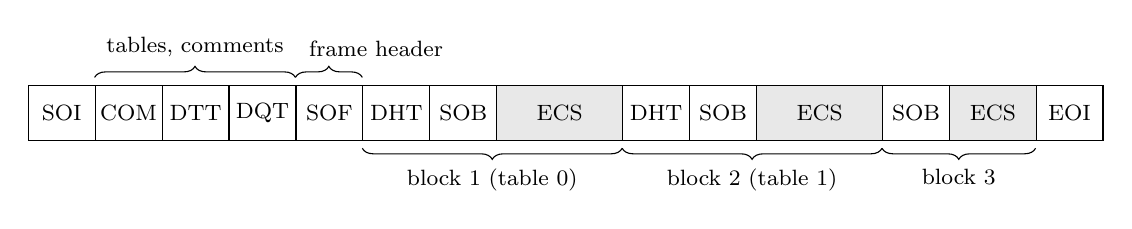
\begin{tikzpicture}[x=1cm,y=1cm,font=\footnotesize,
    seg/.style={draw,minimum height=7mm,inner sep=1pt,anchor=west},
    ecs/.style={seg,fill=gray!18}]
  \def\row#1{%
    \foreach \name/\w/\st [remember=\x as \lastx (initially 0)] in {#1} {
      \pgfmathsetmacro{\x}{\lastx+\w}
      \node[\st,minimum width=\w cm] at (\lastx,0) {\name};
    }}
  \begin{scope}
    \row{\marker{SOI}/0.85/seg, \marker{COM}/0.85/seg, \marker{DTT}/0.85/seg, \marker{DQT}/0.85/seg,
         \marker{SOF}/0.85/seg, \marker{DHT}/0.85/seg, \marker{SOB}/0.85/seg, ECS/1.6/ecs,
         \marker{DHT}/0.85/seg, \marker{SOB}/0.85/seg, ECS/1.6/ecs,
         \marker{SOB}/0.85/seg, ECS/1.1/ecs, \marker{EOI}/0.85/seg}
  \end{scope}
  \draw[decorate,decoration={brace,amplitude=4pt}] (0.85,0.45) -- (3.4,0.45)
    node[midway,above=4pt] {tables, comments};
  \draw[decorate,decoration={brace,amplitude=4pt}] (3.4,0.45) -- (4.25,0.45)
    node[midway,above=4pt,xshift=6mm] {frame header};
  \draw[decorate,decoration={brace,amplitude=4pt,mirror}] (4.25,-0.45) -- (7.55,-0.45)
    node[midway,below=4pt] {block 1 (table 0)};
  \draw[decorate,decoration={brace,amplitude=4pt,mirror}] (7.55,-0.45) -- (10.85,-0.45)
    node[midway,below=4pt] {block 2 (table 1)};
  \draw[decorate,decoration={brace,amplitude=4pt,mirror}] (10.85,-0.45) -- (12.8,-0.45)
    node[midway,below=4pt] {block 3};
\end{tikzpicture}
